\documentclass{article}
\usepackage{amsmath}
\usepackage{listings,lstautogobble}
\usepackage{graphicx}
\usepackage{python}
\lstset{
    frame=single,
    breaklines=true,
    keepspaces=true
}
\usepackage[letterpaper, landscape, margin=1.5in]{geometry}
\begin{document}

\the\textwidth

\section{Introduction}

This document highlights simple usages of the bayesian-framework package used for state estimation, parameter estimation and model selection.. All the functions for the examples are in the file "functions.cpp"

\section{Example 1}

\subsection{Description}
We first look at a bivariate Gaussian distribution denoted by 
\begin{equation}
p(\vec{x}) = \frac{1}{2 \pi } \exp\left( -\frac{\vec{x} \vec{x}^T}{2} \right)
\end{equation}
where the covariance is the identity matrix and the mean is zero. For that first example we compute the evidence using Chib-Jeliazkov and using a quadrature approach. We first need to create the likelihood function in the form of
\begin{equation}
p(\vec{x}) \propto -\frac{\vec{x} \vec{x}^T}{2}
\end{equation}

\begin{lstlisting}
extern "C" double likelihood 
\end{lstlisting}

The necessary files are in the Example-1 folder.


\section{Example 2}

\subsection{Description}
In the first example we perform model selection on a mass-spring-damper system where the mass, the damping and the forcing is known. The stiffness is unknown. The two proposed models are described by 

\begin{align}
\mathcal{M}_1 &:\quad m \ddot{u} + c \dot{u} + k u + k_c u^3 = A \cos( 2 \pi f t ) 						\label{eq:example1:forecast1}  \\
\mathcal{M}_2 &:\quad m \ddot{u} + c \dot{u} + k u + k_c u^3 = A \cos( 2 \pi f t ) + \sigma W(t)		    \label{eq:example1:forecast2}
\end{align}
with measurements
\begin{equation}
d_j = u(t_j) + \varepsilon_j \label{eq:example1:meas}
\end{equation}
where $\varepsilon_j \sim \mathcal(0, \gamma^2)$. To solve the ODE described by Eq.~\eqref{eq:example1:forecast1} there is therefore no need to perform state estimation. The SODE described by Eq.~\eqref{eq:example1:forecast2} is stochastic and linear. State estimation will performed by the Kalman filter. In the code, the Kalman filter is not implemented. EKF will be use instead. For a linear system, EKF is the same as the KF.

%We will use the deterministic system of Eq.~\eqref{eq:example1:forecast1} to generate the measurement. To do so we first need to express Eq.~\eqref{eq:example1:forecast1} in a state space format.
%\begin{equation}
%\begin{bmatrix}
%\dot{x}_1 \\
%\dot{x}_2
%\end{bmatrix} = 
%\begin{bmatrix}
%0 & 1 \\
%-k/m & -c/m 
%\end{bmatrix}
%\begin{bmatrix}
%x_1 \\
%x_2
%\end{bmatrix}
%+ A/m \cos( 2 \pi f t ) \begin{bmatrix}
%0 \\
%1 
%\end{bmatrix}
%\end{equation}
%The next step is to discretize the equation. For this simple system, we can use Euler.
%\begin{equation}
%\begin{bmatrix}
%{x}_{1,k+1} \\
%{x}_{2,k+1}
%\end{bmatrix} = 
%\begin{bmatrix}
%1 & \Delta t \\
%-\Delta t(k/m) & 1- \Delta t(c/m) 
%\end{bmatrix}
%\begin{bmatrix}
%x_{1,k} \\
%x_{2,k}
%\end{bmatrix}
%+ A/m \cos( 2 \pi f t_k )
% \begin{bmatrix}
%0 \\
%1 
%\end{bmatrix} \label{eq:example1:euler}
%\end{equation}
%
%Similarly the stochastic ode described by Eq.~\eqref{eq:example1:forecast2} discretized form is 
%\begin{equation}
%\begin{bmatrix}
%{x}_{1,k+1} \\
%{x}_{2,k+1}
%\end{bmatrix} = 
%\begin{bmatrix}
%1 & \Delta t \\
%-\Delta t(k/m) & 1- \Delta t(c/m) 
%\end{bmatrix}
%\begin{bmatrix}
%x_{1,k} \\
%x_{2,k}
%\end{bmatrix}
%+ \Delta t A/m \cos( 2 \pi f t_k )
% \begin{bmatrix}
%0 \\
%1 
%\end{bmatrix} 
%+ \sqrt{\Delta t} \sigma/m q_k
% \begin{bmatrix}
%0 \\
%1 
%\end{bmatrix} 
%\label{eq:example1:euler2}
%\end{equation}

%Instead of jumping to parameter estimation and model selection, we will look at state estimation. Given a parameter vector, a state estimation run can be by setting the flag $\text{state_estimation}$ in the config file.

%Running the state estimation will produce a log file <model name>-state-estimation.dat. The state estimation file is organized as follows, for each row, the first columns are always the state followed by the covariance, followed by the measurement, the log-likelihood and the time. If there are no measurements a value of $-999$ and $-1999$ is used as a place holder in the data and log-likelihood value. There are repeating time values. After an update step the time doesn't change so both values are shown.



\subsection{Set-up}

Now that we have the discretized formulation to simulate the mass-spring-damper system, we need to code it in functions.cpp. The first 3 lines indicates that we are using the {\em statespace} object and we will be using armadillo to represent the vectors.

%\lstinputlisting[language=C++, firstline=1, lastline=3]{functions.cpp}

The next step is to code  Eq.~\eqref{eq:example1:euler2}

%\lstinputlisting[language=C++, firstline=5, lastline=26]{functions.cpp} 

You can notice that it is not exactly the same function as Eq.~\eqref{eq:example1:euler}. The function implemented in the code is of a mass-spring-damper system that is also perturbed by white noise. However, if $\sigma_g = 0$, it becomes equivalent to the deterministic system. It will be use to both model Eqs.~\eqref{eq:example1:euler} and\eqref{eq:example1:euler2}

\subsubsection{Generating the measurements}

Since we do not have experimental data, we will create our own data. To that end, we will use Eq.~\eqref{eq:example1:meas}. The code to generate the data is in the file {\em gen\_data.cpp}. Depending on what state you are measuring, you will need to change the code accordingly. At the moment only the first state is measured. This may change in the future. The function {\em generateData} will create the measurements based on a specified noise to signal ratio (NSR).

%\lstinputlisting[language=C++, firstline=21, lastline=87]{gen_data.cpp} 

The next step is to compile the code. To do so we first compile {\em functions.cpp}. In the terminal, type
\begin{lstlisting}
make func
\end{lstlisting}
Notice the creation of the file {\em libf.so}. The next step is to compile the generating data file
\begin{lstlisting}
make data
\end{lstlisting}
Notice the creation of {\em data.out}.

We have yet to specify the timestep, for how long the system should be simulated, how many data points, the parameters of the system, etc ... To do this we will write the configuration file {\em genmodels.cfg}. In that file we can specify as many models as we want. For example, the same model could be specified for various set of parameters. Each entry corresponds to one simulation of the system.

%\lstinputlisting[firstline=1, lastline=15]{genmodels.cfg} 

The next table shows the configuration flags and their meaning
\begin{table}[h]
\begin{tabular}{| l | l |}
\hline 
Flag & Description \\
\hline 
name & Name of the model \\
handle & name of the function to simulate the system \\
folder & where the data will be stored. Make sure that the folder exists \\
initialState & Initial state of the system \\
param & Parameters of the system \\
time & How long the system will be simulated \\
dt & timestep \\
dty & measurement timestep \\
NSR & Noise to signal ratio \\
\hline
\end{tabular}
\end{table}

In this case, we will have a data point each $0.1$ second, the MSD is simulated for $10$ seconds, $m = 1kg$, $c = 3.0 N s /m$, $k = 2000 N/m$, $\sigma_g = 2.0$, $A = 400 N$ and $f  = 6 Hz$. Furthermore, $u(0) = 0, \dot{u}(0) = 0$, the time step $\Delta t =  1e-4$ and the NSR is $5\%$.

To generate the data, type in the terminal

\fbox{Note: If you have to make any change to this file, there is no need to recompile the whole package. Simply recompile that file. }

\begin{lstlisting}
mkdir Example1 (note: In case the folder did not exist)
./data.out genmodels.cfg
\end{lstlisting}

To plot the generated measurements

\begin{lstlisting}
cd Example1
python ../../visualization/visualisation.py -d -n x
\end{lstlisting}

Running the previous command, created 3 files in folder {\em Example1}. The file {\em true.dat} contains the true signal from which the measurements are generated, {\em data.dat}  contains 2 rows. The first row is the measurement and the second row contains the time at which they were taken. Finally, {\em variance.dat} is the variance of the measurements. One possible realisation of measurements is given in Fig~\ref{fig:example1data}.

%\begin{figure}[!ht]
%  \centering
%    \includegraphics[width=0.8\textwidth]{./Example1/data.eps}
%      \caption{Data generated for mass-spring-damper system of Example 1.}
%    \label{fig:example1data}
%\end{figure}


This concludes the first part of generating the data. The next part deals with parameter estimation. 
\begin{figure}
\includegraphics[]{./example-2/figs/dense_data.eps}
\end{figure}

\subsubsection{Model selection and parameter estimation}

In {\em functions.cpp}, we will write the proposed model. The proposed model can be different from the generating model but in our case, it will the same. We first propose a deterministic mass spring damper system that will be called {\em example1Model}. This model only has one unknown parameter, we must define the other parameters in the function itself. Each unknown parameter is part of the vector {\em parameter}. In this case the stiffness $k = parameter[0]$. 

%\lstinputlisting[language=C++, firstline=32, lastline=52]{functions.cpp} 

We also need to describe the measurement operator. In this case the noise operator doesn't include the additive Gaussian noise.
%\lstinputlisting[language=C++, firstline=54, lastline=58]{functions.cpp} 

The final part is to describe the proposed state space for that model {\em example1StateSpace}.
%\lstinputlisting[language=C++, firstline=72, lastline=72]{functions.cpp} 

The next step is to compile the code. To do so we first compile {\em functions.cpp}. In the terminal, type
\begin{lstlisting}
make func
\end{lstlisting}

The next step is the configuration file for the proposed models {\em propmodels.cfg}. For this example, we only propose 1 model. For model selection, we would need to propose multiple models.

%\lstinputlisting[firstline=6, lastline=19]{example1.cfg} 

The next table shows the configuration flags and their meaning
\begin{table}[h]
\begin{tabular}{| l | l | l |}
\hline 
Flag & Description & Default value \\
\hline 
run & Flag to indicate to use this model & \\
state\_estimator & What state estimator to use & \\
name & Name of the model & \\
handle & name of the state space to simulate the system & \\
folder & where the data will be stored. Make sure that the folder exists & \\
data & Name of the data file &  \\
initialState & Initial state of the system & \\
param & Initial parameters (starting point the MCMC chain) & \\
method & MCMC method & \\
dt & timestep & \\
measurementCov & measurement covariance filename & \\
prior & parameter prior & \\
\hline
\end{tabular}
\end{table}


Before running the chains, you can do a simple optimization like Nelder-Mead to find a good starting point for the MCMC chain. Better optimization methods will be provided in future versions. To do so
\begin{lstlisting}
make opt
mpirun -np <NP> ./opt.out example1.cfg
\end{lstlisting}

To run the MCMC chains
\begin{lstlisting}
make main
mpirun -np 2 ./run.out example1.cfg
\end{lstlisting}



\subsection{Results}

Before looking the results it is always a good idea to take a look at the MCMC chains. A visual inspection will confirm if the chain properly mixed. If it did not, tweak the MCMC parameters. You can also use the MAP as the starting point for better mixing. In some cases the chain might never mix for a ill-posed problem.

To visualize the results 
\begin{lstlisting}
cd Example1
python ../../visualization/visualisation.py -i MSD-DET.dat -n k -b 0.3
python ../../visualization/visualisation.py -i MSD-EKF.dat -n k -n \sigma -b 0.3 -b 0.3
\end{lstlisting}
This will create multiple figures presented below

\begin{figure}
\includegraphics[]{./example-2/figs/k.eps}
\end{figure}

\begin{figure}
\includegraphics[]{./example-2/figs/kc.eps}
\end{figure}

\begin{figure}
\includegraphics[]{./example-2/figs/sigma.eps}
\end{figure}


The log of the evidence is recorded in the files MSD-EKF-logevidence.dat and MSD-DET-logevidence.dat.


For this simple example, we can compute the posterior without using MCMC.

\section{Example 3}

In this example, we use the filters to perform state estimation. We compare EKF, EnKF and the bootstrap particle filter.
We first generate the measurements.
\begin{lstlisting}
cd example-3
./data.out genmodels.cfg
\end{lstlisting}
The measurements are shown 
\begin{figure}
\centering
\includegraphics[scale=1.0]{./example-3/figs/data.eps}
\caption{Synthetic measurements used for Example 3}
\end{figure}

\begin{figure}
\centering
\includegraphics[scale=1.0]{./example-3/figs/state_estimation_ekf.eps}
\caption{State Estimation using EKF}
\end{figure}

\begin{figure}
\centering
\includegraphics[scale=1.0]{./example-3/figs/state_estimation_enkf.eps}
\caption{State Estimation using EnKF}
\end{figure}

\begin{figure}
\centering
\includegraphics[scale=1.0]{./example-3/figs/state_estimation_pf_serial.eps}
\caption{State Estimation using PF-SERIAL}
\end{figure}

\begin{figure}
\centering
\includegraphics[scale=1.0]{./example-3/figs/state_estimation_pf_mpi.eps}
\caption{State Estimation using PF-MPI}
\end{figure}

\begin{figure}
\centering
\includegraphics[scale=1.0]{./example-3/figs/state_estimation_error.eps}
\caption{Error}
\end{figure}


\end{document}